\chapter{St.\,Ignucius}

Das Maui High Performance Computing Center befindet sich in einem einstöckigen Gebäude in den sandigen Hügeln über der Stadt Kihei. Eingefasst in eine Multi-Millionen-Dollar-Umgebung und das Multi-Millionen-Dollar-Anwesen des Silversword Golf Course, scheint das Center die ultimative Verschwendung von Staatsgeldern im wissenschaftlichen Bereich zu sein. Ganz anders als im klotzigen, sterilen Rahmen des Tech Squares oder selbst die ausgedehnten Forschungsmetropolen Argonne in Illinois und Los Alamos in New Mexico wirkt das MHPCC wie ein Ort, an dem die Wissenschaftler mehr Zeit in ihre Bräune investieren als in ihre Forschungsprojekte als Postdoktoranden.

Das Bild entspricht nur zum Teil der Wahrheit. Obwohl die Forscher am MHPCC die örtlichen Freizeitgelegenheiten nutzen, nehmen sie auch ihre Arbeit ernst. Laut \href{http://Top500.org}{Top500.org} schafft der Supercomputer\comment{IBM SP Power3 im MHPCC 837 Milliarden} auf Basis von Dells PowerEdge-M610-Blades maximal 80,6\,Billionen Gleitkommaoperationen (TFlops) pro Sekunde, was ihm den 114.\,Platz\footnote{Stand: 03.08.2011} auf der Liste der 500 leistungsfähigsten Supercomputer einbringt.\comment{einem der 25 leistungsstärksten Rechner} Die Rechenzeit des in Besitz der University of Hawaii und der U.S. Air Force stehenden Computers wird zwischen den Berechnungen im Bereich von Militärlogistik und Hochtemperaturphysik geteilt.

Einfach gesagt ist das MHPCC ein einzigartiger Ort; ein Ort, an dem die kopflastige Kultur der Wissenschaft und Technik und die entspannte Kultur der Hawaiischen Inseln in völliger Harmonie koexistieren. Ein Slogan auf der Webseite von 2000 fasst es so zusammen: "`Computing in paradise"'.

Es ist nicht die Szenerie, in der man Richard Stallman erwarten würde, ein Mann, der, wenn er den wunderschönen Blick auf den nahe gelegenen Kanal hat, die Kritik äußert\comment{when taking in the beautiful view of the nearby Maui Channel through the picture windows of a staffer's office}: "`Zu viel Sonne."' Dennoch muss Stallman als Abgesandter eines anderen Computerparadieses eine Botschaft überbringen, selbst wenn es bedeutet, dass seine Hackeraugen dem grellen Sonnenlicht ausgesetzt werden.

Der Konferenzraum ist schon fast voll, als ich ankomme, um Stallmans Rede zu lauschen. Die Geschlechterverteilung ist etwas besser als bei der New Yorker Rede, 85\% männlich, 15\% weiblich\comment{, but not by much}. Fast die Hälfte der Zuhörerschaft trägt khakifarbene Hosen und Golfshirts mit Logos. Die andere Hälfte scheint einheimisch gekleidet. In den farbenfrohen blumenbedruckten Shirts, die in dem Teil der Welt so populär sind, treten ihre Gesichter in einem tiefen Ockerton hervor. Das einzige Anzeichen für den Geek-Status sind hier die Gadgets: Nokia-Mobiltelefone, Palm Pilots und VAIO-Laptops.

Unnötig zu erwähnen, dass Stallman vorne im Rednerbereich in seinem einfarbigen blauen T-Shirt, brauner Polyesterhose und weißen Socken auffällt wie ein bunter Hund. Das fluoreszierende Licht im Konferenzsaal hebt die ungesunde Farbe seiner sonnenhungrigen Haut hervor.\footnote{RMS: Die Vorstellung, dass Haut nach Sonne hungern könne, oder dass Blassheit "`ungesund"' sei, ist eine gefährliche Desinformation; sich von der Sonne fernzuhalten, kann nicht schaden, solange man genug Vitamin D hat. Was die Haut wirklich schädigen kann, oder einen sogar umbringen, ist das exzessive Aussetzen an Sonnenlicht.} Sein Bart und seine Haare reichen aus, um auch auf den kühlsten hawaiischen Hals Schweißperlen zu treiben. Nur wenn Stallman noch dazu "`Festlandbewohner"' auf die Stirn tätowiert hätte, sähe er noch fremdartiger aus. [RMS: Ist es irgendetwas Schlechtes, anders als die anderen auszusehen?]

Während Stallman vorn herumwerkelt, richten einige Mitglieder aus der Hörerschaft, die T-Shirts mit dem Logo der Maui FreeBSD Users Group (MFUG) tragen, die Video- und Audio-Ausstattung ein. FreeBSD, ein freier Ableger der Berkeley Software Distribution, der ehrwürdigen akademischen Unix-Version aus den 70ern, ist technisch gesehen ein Konkurrent zum Betriebssystem GNU/Linux. Trotzdem werden in der Hackerwelt die Reden Stallmans mit einer Leidenschaft aufgezeichnet, die an die Grateful Dead und ihre legendäre Armee von Amateur-Archivisten erinnert. Als örtliche Free-Software-Heads liegt es an den MFUG-Mitgliedern, dass die Programmiererkollegen in  Hamburg, Mumbai und Nowosibirsk nicht die neuesten Perlen RMSs Weisheit versäumen.

Der Grateful-Dead-Vergleich ist angemessen. Wenn Stallman die dem Free-Software-Modell inhärenten wirtschaftlichen Möglichkeiten beschreibt, stützt er sich oft auf die Grateful Dead als Beispiel. Mit der Unterstützung ihrer Fans beim Aufnehmen von Live-Konzerten sind die Grateful Dead zu mehr als nur einer Rockgruppe geworden. Sie wurden das Zentrum einer Stammesgruppe, die sich der Musik der Grateful Dead verschreibt. Mit der Zeit wurde diese Anhängerschaft so groß und treu, dass die Band Plattenverträge gemieden und sich nur durch Tourneen und Liveauftritte über Wasser gehalten hat. 1994, im letzten Jahr als Tourgruppe, nahmen die Grateful Dead allein 52 Millionen Dollar mit Ticketverkäufen ein.\footcite[Vgl.][]{gfdgrosses}

Obwohl nur einige Softwareunternehmen einen ähnlichen Erfolg haben erreichen können, ist der Stammesaspekt der Free-Software-Gemeinde in der zweiten Hälfte der 90er einer der Gründe gewesen, die Vorstellung zu akzeptieren, dass die Veröffentlichung des Quellcodes vielleicht etwas Gutes ist. In der Hoffnung, ihre eigenen treuen Gefolgschaften aufzubauen, sind Firmen wie IBM, Sun Microsystems und Hewlett Packard dazu gekommen, den Text der Stallmanschen Free-Software-Botschaft zu akzeptieren, vielleicht sogar ihren Geist. ZDNets Software-Kolumnist Evan Leibovitch beschreibt die GPL als die \textit{Magna Carta} der Computerindustrie und sieht in der wachsenden Neigung zu GNU mehr als nur einen Trend. "`Diese gesellschaftliche Verschiebung lässt die Nutzer wieder die Kontrolle über ihre Zukunft übernehmen"', schreibt Leibovitch. "`Genau wie die \textit{Magna Carta} den britischen Untertanen Rechte gab, forciert die GPL Verbraucherrechte und Freiheiten der Nutzer von Software."'\footcite[Vgl.][]{whosafraid}

Der Stammesaspekt der Free-Software-Gemeinde erklärt auch, warum sich über 40jährige Programmierer, die sonst an Physikprojekten arbeiten würden oder sich im Internet  Bojenmessungen anschauen würden, in einem Konferenzraum\comment{Hörsaal??} versammelt haben, um Stallmans Rede zu hören.

Anders als bei seiner Rede in New York bekommt Stallman keine Ankündigung. Er stellt sich auch nicht selbst vor. Als die FreeBSD-Leute schließlich ihre Aufzeichnungsgeräte am Laufen haben, tritt Stallman einen Schritt nach vorn, fängt einfach an zu reden und übertönt alle anderen Stimmen im Raum.

"`Meistens, wenn Leute die Frage betrachten, welche Regeln die Gesellschaft bei der Benutzung von Software haben sollte, wird diese Frage von Leuten aus Softwarefirmen [aufgeworfen] und sie betrachten die Frage aus einer eigennützigen Perspektive"', eröffnet Stallman seine Rede. "`Welche Regeln können wir allen anderen oktroyieren, damit sie uns einen Haufen Geld bezahlen? Ich hatte das Glück, in den 70ern Teil einer Gemeinschaft von Hackern zu sein, die Software untereinander teilt. Und deswegen sehe ich mir diese Probleme immer gern aus einer anderen Warte an und frage: welche Art von Regeln ermöglichen eine gute Gesellschaft, die für die Leute gut ist, die Teil von ihr sind? Und deshalb komme ich auf völlig verschiedene Antworten."'

Wieder geht Stallman nahtlos zur Parabel über den Xerox-Drucker über, mit derselben Fingerzeiggeste. Auch widmet er dem Namen GNU/Linux ein, zwei Minuten.

%Du/Sie?
"`Einige Leute sagen mir, \glq Warum machst du so viel Aufhebens um deine Anerkennung für das System? Im Endeffekt zählt doch nur, dass das Ziel erreicht ist, und nicht dass du dafür Anerkennung bekommst.\grq{} Na ja, das wäre ein guter Rat, wenn er denn wahr wäre. Es war [aber] nicht das Ziel, ein Betriebssystem zu schaffen; das Ziel ist es, Freiheit unter den Computernutzern zu verbreiten. Und um das zu tun, müssen wir es ermöglichen, alles mit Computern in Freiheit machen zu können."'\footnote{\comment{BLABLA For narrative purposes, I have hesitated to go in-depth when describing Stallman's full definition of software "`freedom."'}Die Webseite des GNU Projects listet folgende vier fundamentale Komponenten:

\index{Freiheiten, Die vier}
\begin{itemize}
  \item Die Freiheit, das Programm ganz nach Wunsch auszuführen, zu jedem Zweck (Freiheit 0).
  \item Die Freiheit, den Quellcode des Programms zu studieren und ihn zu verändern, damit das Programm tut, was man will (Freiheit 1).
  \item Die Freiheit, Kopien des Programms weiterzuverbreiten, um seinem Nächsten zu helfen (Freiheit 2).
  \item Die Freiheit, Kopien seiner modifizierten Version zu verbreiten, damit die ganze Gemeinschaft davon profitieren kann (Freiheit 3).
\end{itemize}

Weitere Informationen findet man in der \cite[][]{freeswdef}.}

Und Stallman ergänzt: "`Es ist noch viel Arbeit zu tun."'

Für einige im Publikum ist das altes Material. Für andere ist es etwas mysteriös. Als ein Mitglied der Golfshirt-Fraktion im Einschlafen begriffen ist, unterbricht Stallman seine Rede und bittet, dass ihn jemanden aufweckt.

"`Jemand hat mal gesagt, meine Stimme wäre beruhigend, und hat gefragt, ob ich eine Art Heiler bin"', sagt Stallman und erntet kurzes Lachen aus der Menge. "`Ich vermute, das heißt, dass ich euch helfen kann, sanft in einen seligen, entspannenden Schlaf zu gleiten. Und einige brauchen [diesen Schlaf]. Ich glaube, ich kann dagegen nichts einwenden. Wenn ihr schlafen müsst, dann lasst euch nicht abhalten."'

Die Rede endet mit einer kurzen Diskussion über Softwarepatente, einer wachsenden Bedrohung in der Softwareindustrie und in der Free-Software-Gemeinde. Wie Napster reflektieren Softwarepatente die heikle Natur der Anwendung von Gesetzen und Konzepten, die für die physische Welt geschaffen sind, auf das reibungslose Universum der Informationstechnologie.

Das Urheberrecht und das Patentrecht funktionieren verschieden und haben völlig verschiedene Auswirkungen auf das Softwareumfeld. Das Urheberrecht auf ein Programm reguliert das Kopieren und die Anpassung des Programmcodes und es steht dem Entwickler des Programms zu. Aber das Urheberrecht deckt keine Ideen ab. Anders gesagt kann ein Entwickler mit dem Urheberrecht vereinbar seine eigenen Funktionen und Befehle implementieren, die er in einem fremden Programm gesehen hat. Diese Aspekte sind Ideen, und keine Äußerungen, und fallen deshalb nicht unter das Urheberrecht.

Es ist ebenso legal – aber sehr schwierig – zu entschlüsseln, wie ein in Binärform vorliegendes Programm funktioniert, und dieselben Ideen und Algorithmen dann selbst zu programmieren. Diesen Vorgang nennt man "`Reverse engineering"'.

Software-Patente funktionieren anders. Laut dem U.\,S. Patent Office können Firmen und Einzelpersonen Patente auf innovative (oder jedenfalls dem Amt unbekannte) Konzepte anmelden. Theoretisch erlaubt das dem Patentinhaber, für die Geheimhaltung der Technik im Gegenzug ein spezielles Monopol mit mindestens 20 Jahren Dauer nach der Anmeldung zu erhalten. In der Praxis ist die Geheimhaltung vor der Allgemeinheit kaum etwas wert, weil die Funktionsweise des Programms oft selbsterklärend ist und auf jeden Fall durch Reverse engineering herausgefunden werden kann. Anders als das Urheberrecht gibt ein Patent seinem Inhaber die Macht, unabhängige Entwicklungen von Software zu unterbinden, die das patentierte Konzept verwenden.

%Patente abgelaufen
In der Softwareindustrie, wo 20 Jahre ein ganzer Lebenszyklus für einen Markt sein können, nehmen Patente eine strategische Rolle ein. Wenn sich früher Unternehmen wie Microsoft und Apple über Urheberrechte und das "`Look and Feel"' verschiedener Technologien bekämpft haben, nutzen heutige Internetunternehmen Patente, um sich einzelne Anwendungen und Geschäftsmodelle abzustecken\comment{stake out}. Das bekannteste Beispiel ist Amazon.coms Versuch im Jahr 2000, den Online-Bestellvorgang  "`One-click"' patentieren zu lassen. Für die meisten Unternehmen sind Softwarepatente jedoch Mittel zur Verteidigung geworden; mit Kreuzlizenzierungsabkommen balancieren sie ihre Patentsammlung gegeneinander aus\comment{in a tense form of corporate detente}. Trotzdem gibt es einige berüchtigte Fälle, in denen Softwareunternehmen bei Verschlüsselungs- und graphischen Algorithmen erfolgreich die Entwicklungen ihrer Konkurrenten erstickt haben. Zum Beispiel fehlten lange Zeit einige Renderingfunktionen für Schriften in freier Software wegen Patenten von Apple.\footcite[Vgl.][]{freetypepat}

Für Stallman verdeutlicht das Thema der Softwarepatente die ständige Notwendigkeit für Hacker, wachsam zu sein. Es unterstreicht auch die Wichtigkeit der politischen Vorteile von freier Software über die Vorteile gegenüber den Rivalen\comment{competitive benefits}. Stallman meint, Wettbewerbsfähigkeit und Preis, zwei Bereiche, in denen freie Betriebssysteme wie GNU/Linux und FreeBSD schon einen deutlichen Vorsprung gegenüber ihren proprietären Gegenstücken haben, sind nebensächlich im Vergleich zu dem wichtigeren Thema der Nutzer- und Entwicklerfreiheit.

Diese Position ist in der Gemeinde umstritten: die Open-Source-Befürworter betonen die funktionellen Vorzüge freier Software mehr als die politischen. Statt die politische Bedeutung freier Programme zu betonen, betonen Open-Source-Befürworter die technische Integrität des Hacker-Entwicklungsmodells. Die Open-Source-Seite argumentiert mit der Stärke der Peer reviews und beschreibt Systeme wie GNU/Linux oder FreeBSD als besser konstruiert, besser geprüft und infolgedessen als vertrauenswürdiger für den Durchschnittsnutzer.

Das soll nicht heißen, der Begriff "`Open Source"' hätte nicht auch seine politischen Implikationen. Für Open-Source-Befürworter erfüllt der Begriff zwei Zwecke. Zum ersten beseitigt er die Verwirrung um das Wort "`free"', das viele Unternehmen als "`umsonst"' deuten. Zum zweiten erlaubt er es den Firmen, das Free-Software-Phänomen auf einer technischen Ebene statt einer ethischen zu beleuchten. Eric Raymond\index{Raymond, Eric|(}, Mitbegründer der Open Source Initiative (OSI) und einer der führenden Hacker, der für den Begriff wirbt, erklärt seine Ablehnung, Stallmans politischem Pfad zu folgen, in einem Essay von 1999 namens \citefield{title}{esrshutup}:

\begin{quote}
RMSs Rhetorik ist sehr verführerisch für Leute wie uns. Wir Hacker sind Denker und Idealisten, die auf Appelle an "`Prinzip[ien]"', "`Freiheit"' und "`Rechte"' Resonanz zeigen. Selbst wenn wir mit kleinen Teilen seines Programms nicht übereinstimmen, wollen wir, dass RMSs rhetorischer Stil wirkt; wir denken, er müsste doch wirken; wir sind meist verblüfft und ungläubig, wenn er bei 95\% der Leute nicht anschlägt, die nicht so ticken wie wir.\footcite[Vgl.][]{esrshutup}
\end{quote}

%Original stellt falsche Behauptung auf -> nicht in Quelle
\comment{Unter diesen 95\%, schreibt Raymond, sind die meisten Manager, Investoren und Nichthacker, die through sheer weight of numbers, tend to decide the overall direction of the commercial software marketplace. }Ohne eine Möglichkeit, diese Leute für sich zu gewinnen, argumentiert Raymond, sind die Programmierer dazu verdammt, ihre Ideologie am Rande der Gesellschaft zu verfolgen:

\begin{quote}
Wenn RMS darauf besteht, dass wir über "`die Rechte von Computernutzern"' sprechen, gibt er uns die verführerische Einladung, alte Misserfolge zu wiederholen. Wir sollten sie ablehnen – nicht, weil seine Prinzipien falsch sind, sondern weil diese Art Sprache im Bezug auf Software einfach niemanden überzeugt außer uns. In Wirklichkeit verwirrt sie und stößt die meisten Leute außerhalb unserer Kultur ab.\footcite[][]{esrshutup}
\end{quote}

Stallman jedoch lehnt Raymonds Prämisse ab:

\begin{quote}
Raymonds Versuch, unser Scheitern zu erklären, ist irreführend, weil wir nicht gescheitert sind. Wir haben große Ziele, und wir haben einen weiten Weg vor uns, aber wir sind auch schon weit gekommen.

Raymonds\index{Raymond, Eric|)} pessimistische Behauptung über die Wertvorstellungen der Nichthacker sind eine Übertreibung. Viele Nichthacker beschäftigen sich mehr mit den politischen Problemen, auf die wir uns konzentrieren, als auf die technischen Vorteile, die Open Source betont. Das schließt auch politische Führungspersönlichkeiten ein, aber nicht in allen Ländern.

Es waren die ethischen Ideale der freien Software, nicht die "`bessere Software"', die die Präsidenten von Equador und Brasilien überzeugt haben, ihre Behörden auf freie Software umzustellen. Sie sind keine Geeks, aber sie verstehen Freiheit.
\end{quote}

Aber die größte Schwäche in den Open-Source-Argumentation ist, laut Stallman, dass sie zu schwächeren Schlüssen kommt. Sie überzeugt viele Leute, einige Programme zu benutzen, die frei sind, aber bietet ihnen keinen Grund, komplett auf freie Software umzustellen. Das gibt ihnen teilweise Freiheit, aber lehrt sie nicht, sie zu erkennen und als solche zu schätzen, und so bleibt es wahrscheinlich, dass sie sie fallenlassen und verlieren. Was passiert zum Beispiel, wenn die Weiterentwicklung freier Software durch Patente blockiert ist?

Die meisten der Open-Source-Befürworter sind genauso lautstark wie Stallman, wenn nicht mehr, wenn es um Softwarepatente geht. Und auch die meisten Entwickler proprietärer Software, weil Patente auch ihre Projekte bedrohen. Jedoch stellt Stallman für den Fall, dass Softwarepatente die Implementierung bestimmter Funktionalität verhindern, das Free-Software-Konzept dem Open-Source-Konzept gegenüber und zeigt auf, worauf beide hinauslaufen.

"`Es liegt nicht daran, dass uns das Talent fehlt, bessere Software zu machen"', sagt Stallman. "`Es liegt daran, dass wir nicht das Recht haben. Jemand hat uns verboten, der Allgemeinheit zu dienen. Was wird dann passieren, wenn die Nutzer diese Lücken in der freien Software bemerken? Wenn sie von der Open-Source-Bewegung überzeugt worden sind, dass diese Freiheiten gut sind, weil sie zu leistungsfähigerer und zuverlässigerer Software führt, dann sagen sie wahrscheinlich: \glq Ihr habt nicht das geliefert, was ihr versprochen habt. Diese Software ist nicht leistungsfähiger. Es fehlt eine Funktion. Ihr habt mich belogen.\grq{} Aber wenn sie sich von der Free-Software-Bewegung haben überzeugen lassen, dass Freiheit selbst wichtig ist, dann werden sie sagen: \glq Was fällt denen ein, mir diese Funktion und außerdem meine Freiheit zu verwehren.\grq{} Und mit dieser Art Reaktion könnten wir die Schläge überleben, die wir einstecken müssen, wenn diese Patente explodieren."'

Wenn man Stallman persönlich seine politische Botschaft übermitteln sieht, kann man kaum etwas Unklares oder Abstoßendes erkennen. Stallmans Äußeres mag unangenehm erscheinen, aber seine Botschaft ist logisch. Als ein Zuhörer fragt, ob die Free-Software-Befürworter mit der Meidung proprietärer Software die Möglichkeit verlieren, mit den neuesten technologischen Fortschritten mitzuhalten, beantwortet Stallman die Frage mit seinen eigenen persönlichen Überzeugungen. "`Ich glaube, dass Freiheit wichtiger ist als bloßer technischer Fortschritt"', sagt er. "`Ich würde immer ein weniger fortschrittliches freies Programm einem fortschrittlicherem unfreien Programm vorziehen, weil ich meine Freiheit nicht für so etwas aufgeben will. Meine Regel ist: Wenn ich es nicht mit dir teilen\comment{austauschen} kann, nehme ich es nicht."'

In den Köpfen derer, die annehmen, Ethik bedeute Religion, untermauern solche Antworten die quasi-religiöse Natur von Stallmans Botschaft. Jedoch gehorcht Stallman keinem Gebot, anders als ein Jude, der koscher lebt oder ein Mormone, der sich weigert, Alkohol zu trinken; er weigert sich einfach, seine Freiheit aufzugeben. In seiner Rede erläutert er die praktischen Voraussetzungen: ein proprietäres Programm nimmt einem die Freiheit, und wenn man Freiheit will, muss man das Programm ablehnen.

Zu seiner persönlichen Entscheidung, freie statt proprietäre Software zu benutzen, hofft Stallman, werden auch andere kommen. Wie es bei Software-Evangelisten üblich ist, vermeidet Stallman es, den Zuhörern diese Überzeugungen aufzudrängen. Trotzdem weiß kaum jemand nach einer Stallman-Rede nicht, wo der wahre Pfad zur Software-Rechtschaffenheit liegt.

Als ob er diese Botschaft klarmachen wollte, akzentuiert Stallman seine Rede mit einem ungewöhnlichen Ritual. Er zieht eine schwarze Robe aus einer Plastiktüte und zieht sie an. Dann zieht er eine blanke braune Festplattenscheibe hervor und setzt sie sich auf. Die Menge lacht verwundert.

%XXX oder Kirche Emacs' / Emacs-Kirche?
"`Ich bin Sankt IGNUcius von der Kirche von Emacs\,"',\index{St.\,IGNUcius|(}\index{Emacs, Church of|(} sagt Stallman und hebt seine rechte Hand für eine Segnungsgeste. "`Gesegnet sei dein Computer, mein Kind."'

\begin{figure}[ht] \centering
  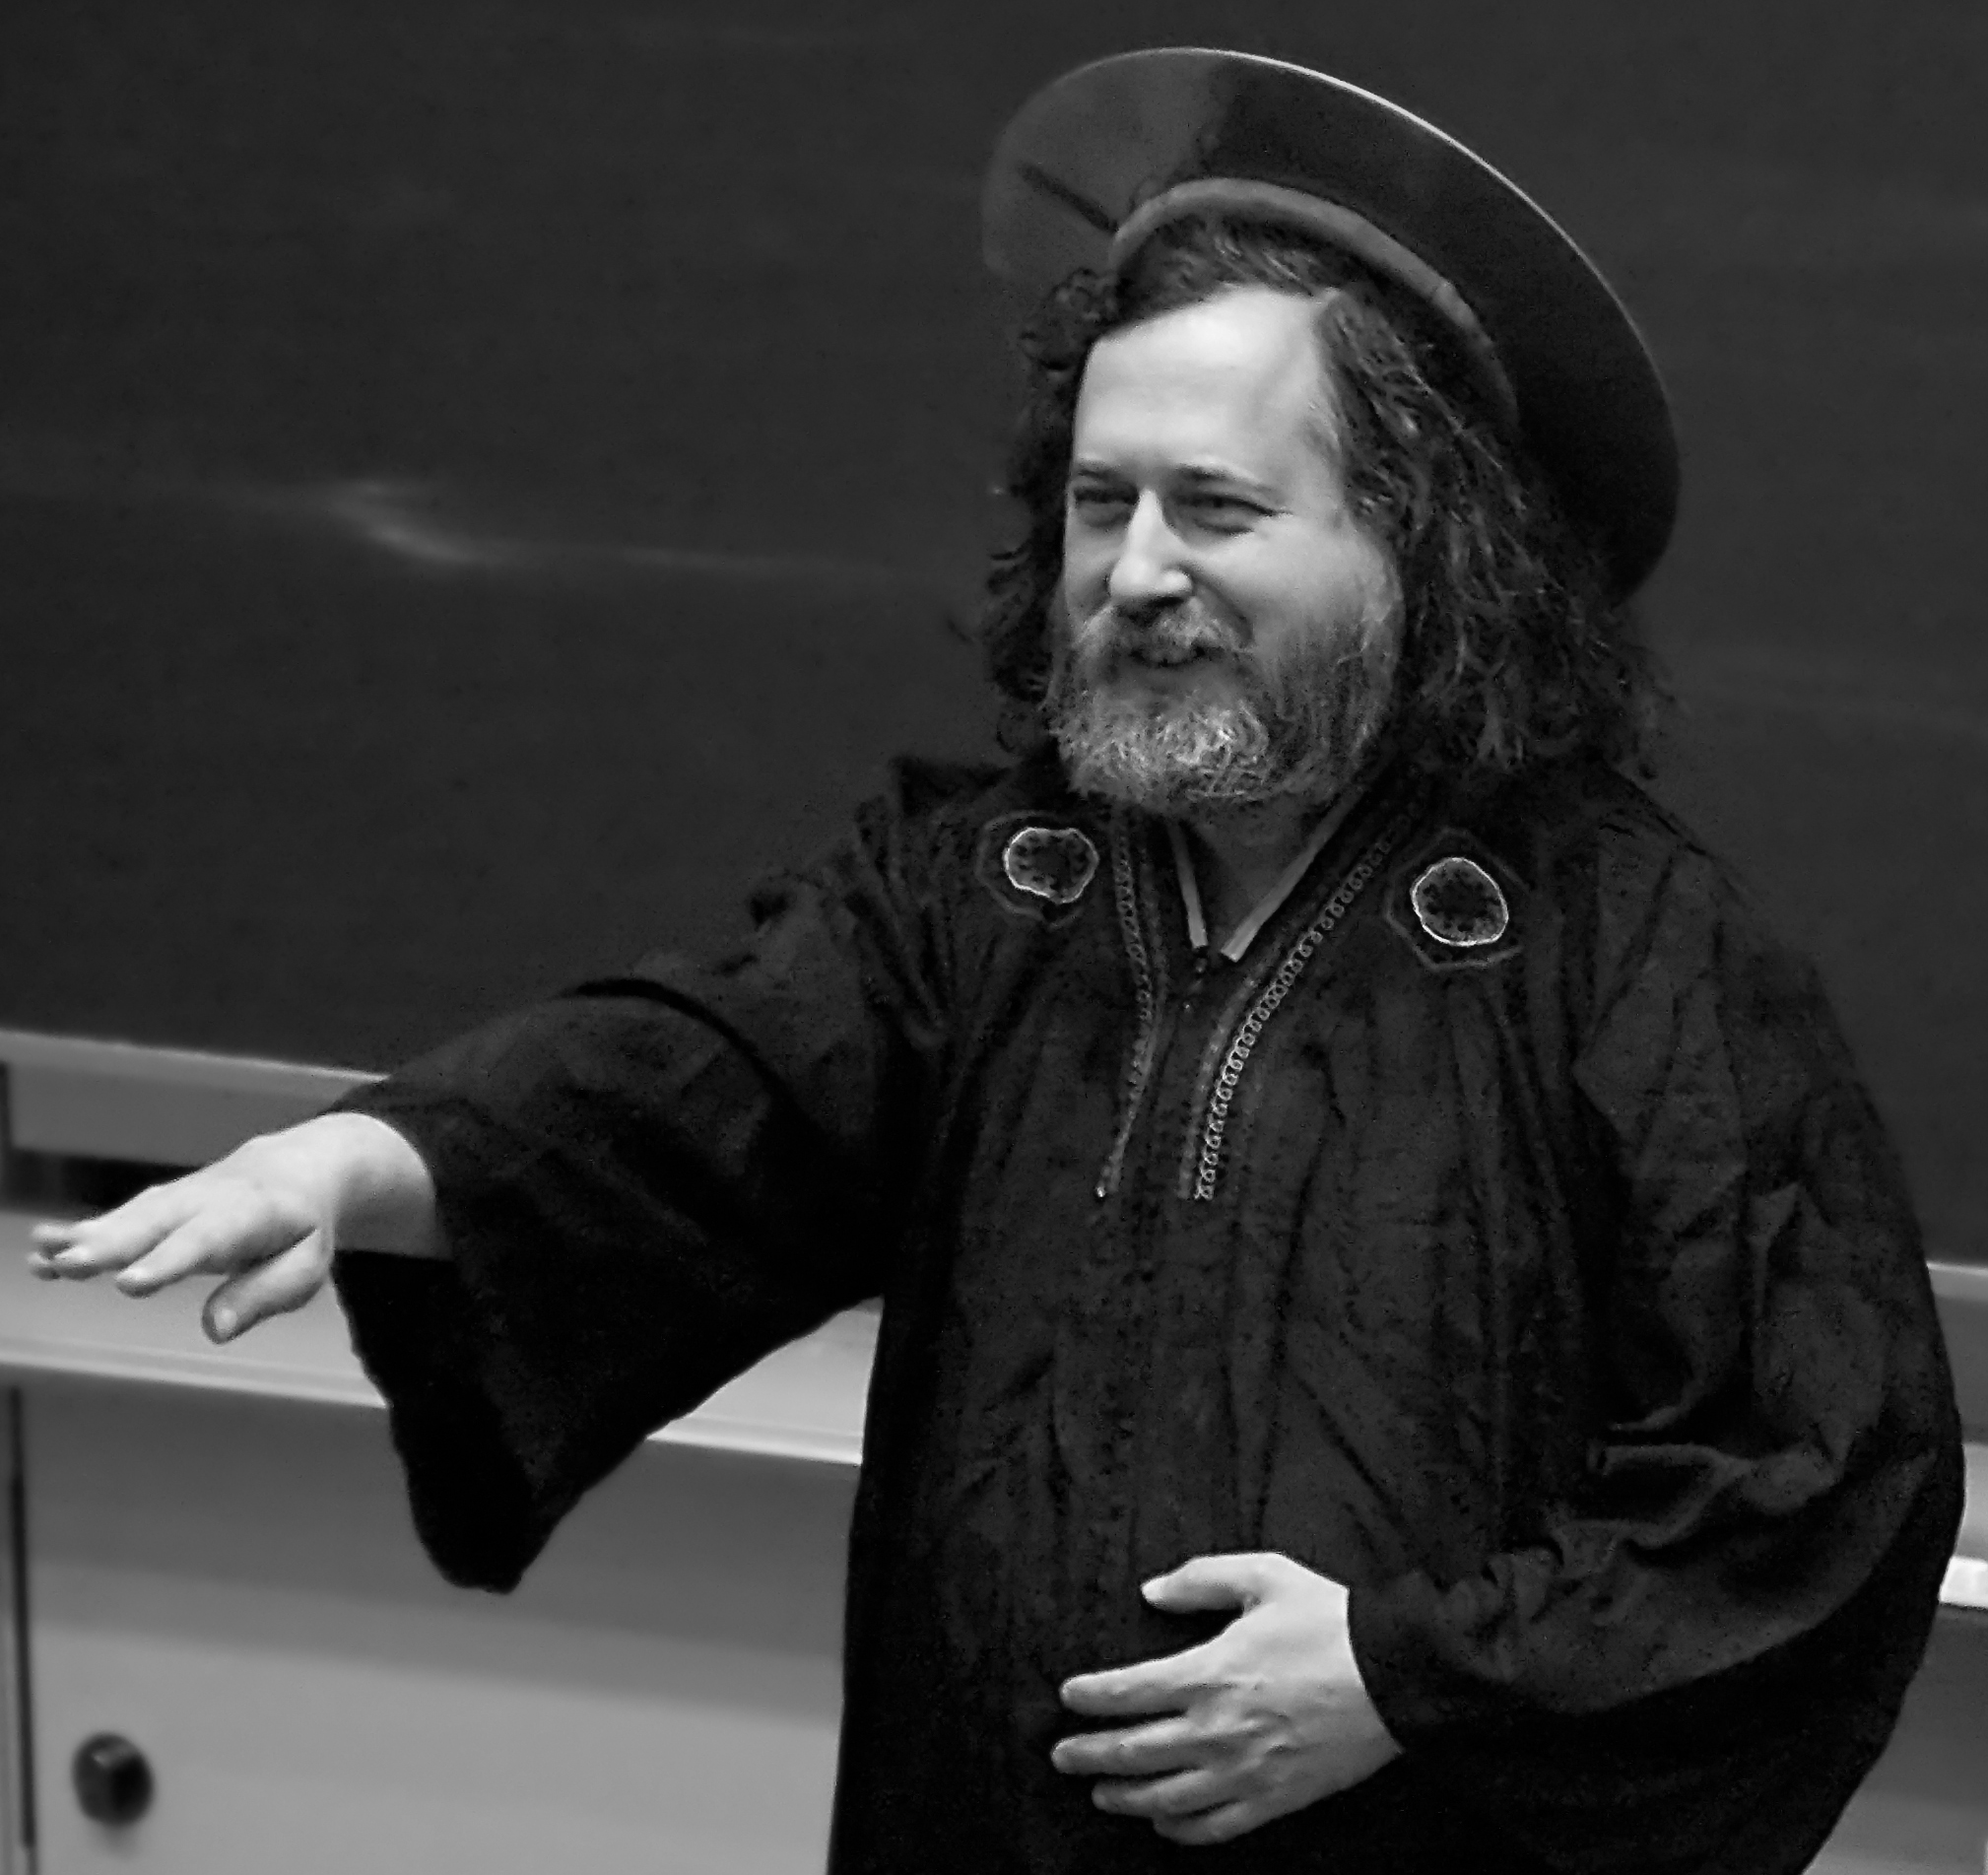
\includegraphics[width=0.7\textwidth]{stignucius}
  \caption{\small Stallman als St.\,IGNUcius verkleidet. Photo: Stian Eikeland, Bergen, 19. Februar 2009.}
\end{figure}

Das Gelächter schlägt nach einigen Sekunden in tosenden Beifall um. Unter dem Beifall bewegt Stallman seinen Kopf in das Licht einer Deckenlampe und sein Heiligenschein fängt an zu leuchten. Für einen kurzen Moment ähnelt Stallman einer russischen Ikone.

"`Emacs war ursprünglich ein Texteditor"', sagt Stallman\comment{, explaining the getup}. "`Schließlich wurde es eine Lebensweise für viele und für einige eine Religion. Wir nennen diese Religion die Kirche von Emacs."'

Der Sketch ist ein unbeschwerter Moment der Selbstparodierung, ein humorvoller Konter gegen die vielen Leute, die Stallmans Form der Softwareaskese als verhüllten religiösen Fanatismus ansehen. Außerdem ist er der Klang des Unausweichlichen\comment{ XXX It is also the sound of the other shoe dropping – loudly}. Als ob Stallman mit dem Anlegen der Robe und dem Aufsetzen des Heiligenscheins seine Hörer endlich vom Haken lässt, wenn er sagt "`Ihr könnt ruhig lachen. Ich weiß, dass ich seltsam bin."'  [RMS: Es ist ungehobelt, über jemanden zu lachen, weil er eigenartig ist, und es ist nicht meine Absicht, das zu entschuldigen. Aber ich hoffe, dass Leute über meine IGNUcius-Comedy-Nummer lachen.]

%erneutes Zitierversagen im Original
Als wir später die Figur des St.\,IGNUcius diskutieren, sagt Stallman, sie sei ihm 1996 eingefallen, lange nach der Schöpfung von Emacs, aber schon lange vor dem Aufkommen von "`Open Source"' und dem folgenden Kampf um die Vorherrschaft in der Hackergemeinde. Zu der Zeit, sagt Stallman, wollte er sich "`über [sich] selbst lustig machen"', um seine Zuhörer zu erinnern, dass er trotz seiner Sturheit nicht der Fanatiker ist, den einige aus ihm machen. Erst später, ergänzt Stallman, hätten andere die Figur als einfache Möglichkeit aufgegriffen, um seinen Ruf als Software-Ideologen hochzuspielen, wie Eric Raymond\index{Raymond, Eric|(} in einem Interview auf Linux.com im Jahr 1999:

\begin{quote}
Wenn ich sage, RMS kalibriert das, was er tut, will ich ihn nicht herabsetzen oder ihn anschuldigen, unaufrichtig zu sein. Ich meine damit, dass er wie alle guten Sprecher eine schauspielerische Ader hat. Manchmal auch bewusst – haben Sie ihn schon mal in seinem St.-IGNUcius-Aufzug gesehen, wie er mit einer Festplattenscheibe auf dem Kopf Software segnet? Meistens ist es unbewusst; er hat einfach gelernt, welches Ausmaß an reizendem Stimulus funktioniert, um das Interesse aufrecht zu halten, (meistens) ohne dass die Leute durchdrehen.\comment{freak out XXX}\footcite[Vgl.][]{esrint}
\end{quote}

Stallman stimmt Raymonds\index{Raymond, Eric|)} Analyse nicht zu. "`Es ist einfach nur meine Art, mich selbst durch den Kakao zu ziehen."', sagt er. "`Der Umstand, dass andere es als irgendetwas mehr ansehen, ist ein Zeichen ihrer Agenda, nicht meiner."'

%hack Schmierenkomödiant
Trotzdem gibt Stallman zu, ein Amateurschauspieler zu sein. "`Machen Sie Scherze?"' sagt er an einer Stelle. "`Ich liebe es, im Mittelpunkt zu stehen."' Um das auszuleben, sagt Stallman, sei er einmal den Toastmasters\index{Toastmasters} beigetreten, einer Organisation, die ihren Mitgliedern hilft, ihre Fähigkeiten im öffentlichen Reden zu verbessern, und Stallman empfiehlt sie wärmstens weiter. Er besitzt eine Bühenpräsenz, die die meisten Theaterdarsteller neidisch machen würde und fühlt eine Verbindung zum Varieté\comment{vaudevillians} aus vergangenen Zeiten. Einige Tage nach der Rede am Maui High Performance Computing Center spiele ich auf die "`Aufführung"' zur LinuxWorld 1999 an und frage Stallman, ob er einen Groucho-Marx-Komplex\index{Marx, Groucho} hat – d.\,h. keinem Club zugehören zu wollen, der ihn als Mitglied hat.\footnote{RMS: Williams missinterpretiert Grouchos berühmte Bemerkung in eine psychologische Richtung. Sie war als Hieb gegen den offenen Antisemitismus vieler Clubs gedacht, welcher der Grund war, warum sie ihn nicht als Mitglied haben wollten. Ich habe es auch nicht verstanden, bis meine Mutter es mir erklärt hat. Williams und ich sind zu einer Zeit aufgewachsen, in der der Fanatismus sich ins Verborgene verschoben hat, und es gab keinen Grund, Kritik daran in Humor zu verhüllen wie Groucho.} Stallman hat sofort eine Antwort: "`Nein, aber ich bewundere Groucho Marx in vieler Hinsicht und ich bin auch inspiriert von ihm in einigen Dingen, die ich sage. Aber ich bin auch in gewisser Hinsicht von Harpo inspiriert."'

% TODO Satz 2, 3 streichen / umformulieren
Der Einfluss von Groucho Marx ist deutlich in seiner lebenslangen Vorliebe für Wortwitze erkennbar. Andererseits sind Wortwitze und -spiele auch eine Eigenart vieler Hacker. Der vielleicht grouchoeskeste Zug an Stallmans Persönlichkeit aber ist seine trockene Art, auf die er seine Witze abliefert. Die meisten kommen so klandestin – ohne einen Hauch einer hochgezogenen Augenbraue oder Lächeln – man fragt sich fast, ob Stallman mehr über seine Hörerschaft lacht als sie über ihn.

Wenn man die Mitglieder des Maui High Performance Computer Centers über die St.-IGNUcius-Persiflage lachen sieht, verschwinden solche Gedanken. Obwohl es nicht gerade eine Standup-Nummer ist, hat Stallman doch das Zeug, einen Raumvoll Ingenieure zum Lachen zu bringen. "`Um ein Heiliger in der Kirche von Emacs zu sein, muss man nicht zölibatär leben, aber man muss sich einem Leben in moralischer Reinheit verpflichten"', erzählt er dem Auditorium in Maui. "`Man muss die bösen proprietären Betriebssysteme von all seinen Computern austreiben und dann ein vollkommen freies Betriebssystem installieren. Und dann nur freie Software darauf installieren. Wenn man diese Verpflichtung eingeht und danach lebt, dann wird man auch ein Heiliger in der Kirche von Emacs und man bekommt seinen Heiligenschein."'

%Schahāda
%Marienkult-Übersetzung funktioniert nicht
Der St.-IGNUcius-Sketch endet mit einem Insiderwitz. Auf den meisten Unix-Systemen und den unixoiden Ablegern ist der Hauptgegner von Emacs vi (sprich: V-I), ein Texteditor vom ehemaligen UC-Berkeley-Studenten und Mitbegründer sowie bis 2003 wissenschaftlicher Leiter bei Sun Microsystems, Bill Joy. Bevor er seinen "`Heiligenschein"' lüpft, frotzelt Stallman über das Konkurrenzprogramm. "`Manchmal fragen mich Leute, ob es in der Kirche von Emacs eine Sünde ist, vi zu benutzen"', sagt er. "`Eine freie Version von vi zu nutzen ist keine Sünde; sondern Buße. Frohes Hacken."'\footnote{Der Gottesdienst hat sich seit 2001 weiterentwickelt. Nutzer können der Kirche beitreten, wenn sie das Glaubensbekenntnis aufsagen: "`Es gibt kein System außer GNU und Linux ist einer seiner Kernel."' Stallman erwähnt manchmal eine religiöse Zeremonie namens Foobar Mitzwa, das Große Schisma zwischen den konkurrierenden Emacs-Versionen, und den Kult um die Jungfrau von Emacs (was sich auf jede Person bezieht, die noch nicht Emacs beherrscht).\footnotemark{} Außerdem kennzeichnet "`vi vi vi"' den Editor des Teufels\comment{Tieres}. Seine neueste Schöpfung ist die "`Emacs-Pilgerfahrt"', bei der alle Befehle von Emacs in alphabetischer Reihenfolge ausgeführt werden.}
\footnotetext{Nach Protesten wegen seiner Keynote auf dem Gran Canaria Desktop Summit 2009 hat Stallman die Definition auf beide Geschlechter erweitert.\comment{"`Um solche Missverständnisse in Zukunft zu vermeiden, habe ich seit August den Witz so geändert, dass eine Emacs-Jungfrau beiderlei Geschlechts sein kann."'} \cite[Vgl.][]{rmssexism}.}

Nach der Beantwortung der Fragen sammeln sich einige Zuhörer um Stallman. Einige bitten um Autogramme. "`Ich signiere das"', sagt Stallman, und hält den Ausdruck der GPL einer Frau hoch, "`aber nur wenn Sie mir versprechen, den Begriff GNU/Linux statt Linux zu verwenden"' (wenn man sich auf das System bezieht) "`und all Ihren Freunden sagen, dass sie das auch tun sollen."'

Die Bemerkung bestätigt eine persönliche Beobachtung. Anders als Bühnenschauspieler und politische Figuren hat Stallman keinen "`Ausschalter"'. Abgesehen von der Figur des Heiligen IGNUcius\index{St.\,IGNUcius|)}\index{Emacs, Church of|)} ist der Ideologe hinter der Bühne so wie auf der Bühne. Später an diesem Abend, als während eines Tischgesprächs ein Programmierer seine Neigung zu "`Open-Source"'-Programmen erwähnt, tadelt Stallman im Kauen seinen Tischgenossen: "`Sie meinen freie Software. Das ist die korrekte Bezeichnung."'

Während der Beantwortung der Publikumsfragen gibt Stallman zu, manchmal den Pädagogen zu spielen. "`Es gibt viele Leute, die sagen \glq Lasst uns erst die Leute bitten, der Gemeinde beizutreten, und sie dann über die Freiheit belehren.\grq{} Und das könnte eine vernünftige Strategie sein, aber de facto wirbt fast jeder Leute für die Gemeinde an, aber kaum jemand erklärt ihnen dann [ihre] Freiheit, wenn sie beigetreten sind."'

Im Ergebnis, sagt Stallman, hätte man dann so etwas wie eine Stadt in der Dritten Welt. "`Man hat Millionen Leute, die dahin ziehen und Barackensiedlungen bauen, aber niemand arbeitet an Schritt zwei: sie aus diesen Barackensiedlungen herauszuholen. Wenn Sie es für eine gute Strategie halten, über Softwarefreiheit zu sprechen, dann beteiligen Sie sich bitte bei Schritt zwei. Es arbeiten schon viele an Schritt eins. Wir brauchen mehr Leute, die an Schritt zwei arbeiten."'

An "`Schritt zwei"' zu arbeiten, bedeutet, dass man klarmacht, dass Freiheit das Kernthema der Free-Software-Bewegung ist, nicht die Akzeptanz [der Software selbst]. Diejenigen, die die proprietäre Softwareindustrie von innen reformieren wollen, sind auf dem Holzweg. "`Änderungen von innen sind riskant"', sagt Stallman. "`Wenn man nicht gerade auf der Ebene Gorbatschows arbeitet, wird man neutralisiert."'

Hände gehen hoch. Stallman weist auf ein Mitglied der Fraktion der Golfshirtträger. "`Wie, schlagen Sie vor, soll man ohne Patente auf Wirtschaftsspionage reagieren?"' – "`Also, diese zwei Fragen haben wirklich nichts miteinander zu tun"' – "`Aber ich meine, wenn jemand die Software einer anderen Firma stehlen will."'

Stallman weicht zurück wie von Giftgas getroffen. "`Moment mal"', sagt Stallman. "`Stehlen? Es tut mir leid, da sind so viele Vorurteile in dieser Aussage, dass ich nur sagen kann, dass ich diese Vorurteile ablehne."' Dann geht er auf die Essenz der Frage ein. "`Firmen, die unfreie Software und andere Dinge entwickeln, haben ganz, ganz viele Geschäftsgeheimnisse und das wird sich wahrscheinlich nicht ändern. Früher – selbst in den 80ern – war dem Großteil der Programmierer nicht bewusst, dass es Softwarepatente überhaupt gibt und haben sich nicht darum gekümmert. Es war so, dass die Leute die interessanten Ideen veröffentlicht haben, und wenn sie nicht zu der Free-Software-Bewegung gehörten, haben sie die kleinen Details geheimgehalten. Und jetzt patentieren sie diese groben Konzepte und halten die kleinen Details geheim. Also haben bei dem, was Sie beschreiben, Patente wirklich keine Auswirkungen, so oder so."'

"`Aber es wirkt sich nicht auf ihre Veröffentlichung aus [der der Ideen]"', springt ein weiterer Zuhörer ein, seine Stimme schwindet schon fast am Anfang des Satzes.

"`Doch, das tut es"', sagt Stallman. "`Ihre Veröffentlichung schreibt einem vor, dass das eine Idee ist, die für den Rest der Gemeinschaft für 20 Jahre tabu ist. Und was zur Hölle soll das bringen? Außerdem haben sie sie so schwer verständlich geschrieben, um die Idee zu verschleiern und das Patent so umfassend wie möglich zu machen, dass es im Grunde nutzlos ist, sich die veröffentlichten Informationen anzusehen, um [daraus] etwas zu lernen. Der einzige Grund, sich Patente anzuschauen, ist, um die schlechte Nachricht zu sehen, was man nicht mehr machen kann."'

Es wird still unter der Zuhörerschaft. Die Rede, die um 3:15 angefangen hat, nähert sich dem Abpfiff um 5:00 und die meisten Zuhörer rutschen schon ungeduldig auf ihren Stühlen herum, hoffen, früh ins Wochenende starten zu können. Stallman nimmt die Müdigkeit wahr, schaut schnell im Raum umher und bringt den Vortrag zu Ende. "`Es sieht so aus, als ob wir fertig sind"', sagt er, gefolgt von einem "`zum ersten, zum zweiten, zum dritten"' wie ein Auktionator\comment{, to flush out any last-minute questioners}. Nachdem sich niemand zu Wort meldet, verabschiedet Stallman sich mit einem klassischen Schlusssatz.

"`Frohes Hacken."'